\section{Interaktion der Komponenten}
Auf Basis der Use Cases aus der Analyse wird in diesem Kapitel die Interaktion der einzelnen Komponenten aus Kapitel 1 betrachtet. \\
Dabei liegt der Fokus vor allem auf der Interaktion zwischen dem \emph{Robot} und dem \emph{Server}, sowie dessen Austausch mit dem \emph{Hospital} und der \emph{TaxiApp}. 
Die Abläufe innerhalb der Komponenten werden dann in Kapitel 8 näher spezifiziert. \\
Zunächst soll der allgemeine Ablauf der Kommunikation spezifiziert werden, bevor auf die konkreten Use Cases eingangen wird.

\subsection*{Kommunikation zwischen Server und RobotUnit}
Zur bidirektionalen Kommunikation zwischen \emph{Server} und \emph{RobotUnit} werden \emph{Remote Procedure Calls} (RPC) eingesetzt. Damit ist der \emph{Server} (respektive \emph{RobotUnit}) in der Lage auf der jeweils anderen Komponente Methoden aufzurufen und deren Rückgabewert zu verwenden. \\ \\
Der Ablauf ist in Abbildung \ref{SequenzDiagrammRPC} dargestellt. \\
Möchte der \emph{Invoker} einen RPC ausführen, wird aus dem gewünschten Methodenaufruf durch Serialisierung des Methodennames und der Parameter eine \texttt{callMessage} erzeugt, die dem \emph{Processor} übermittelt wird. Zur Übermittlung (3. und 4.) wird die im Interface \emph{IWlanAdapter} definierte Methode \texttt{send(message)} aufgerufen. Auf \emph{Processor} Seite wird über \emph{IMessageHandler} die Methode \texttt{handleIncomingMessage(callmessage)} aufgerufen. \\
Nach der Deserialisierung findet der lokale Methodenaufruf statt (\texttt{5: callLocalProcedure}). Der Rückgabewert wird dem InvokerNetworkAccess serialisiert übermittelt. Dies geschieht analog zur oben dargestellten Kommunikation, allerdings in die Rückrichtung. Der \emph{Invoker} deserialisiert die Antwort und teilt sie der aufrufenden Methode als Rückgabewert mit.
\begin{figure}[H]
	\centering
	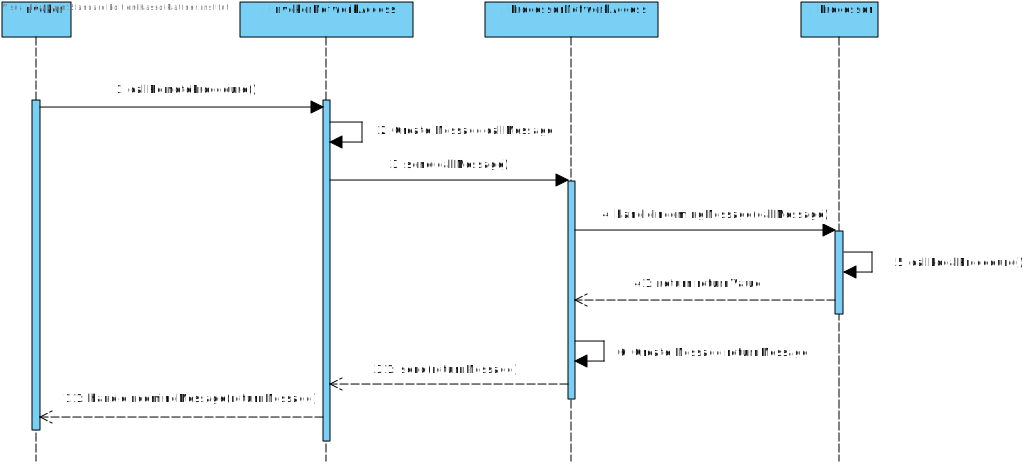
\includegraphics[height=0.85\textwidth, angle=90]{img/2-Entwurf-Communication_RPC}
	\caption{Sequenzdiagramm für einen abstrakten \emph{Remote Procedure Call (RPC)}}
	\label{SequenzDiagrammRPC}
\end{figure}

\subsection*{Interaktion zwischen TaxiApp, Server und RobotUnit}

Der Use Case \texttt{Receive Order} (Use Case 1.1) ermöglicht es \emph{Usern} (Taxikunden und \emph{Hospital}), Anfragen zu stellen, um ein Taxi oder einen Krankentransporter anzufordern. Dabei wird zwischen den \emph{Usern} unterschieden, um die Anfragen des \emph{Hospitals} priorisiert zu behandeln.\\
Zuerst wird auf die Interaktion mit Kunden der \emph{TaxiApp} eingegangen, anschließend wird die Kommunikation mit dem \emph{Hospital} thematisiert. \\ \\

Die Abbildung \ref{SequenzDiagrammInteraktionTaxi} zeigt in einem Sequenzdiagramm den Ablauf der Kommunikation zwischen der \emph{TaxiApp}, dem \emph{Server} und den \emph{RobotUnits}.\\ \\
Die \emph{TaxiApp} ruft zur Implementierung des Use Cases 1.1 auf dem \emph{Server} die im Interface \emph{ITaxiAppUserInputHandler} definierte Methode \texttt{orderTaxi(source, destination)} im ersten Schritt auf, um ein Taxi zu bestellen. \\
Der Server prüft daraufhin die Verfügbarkeit einer \emph{RobotUnit}, indem er im Folgeschritt probiert über \texttt{chooseRobot(task)} eine \emph{RobotUnit} zu wählen. Diese Methode greift u.a. auf die \texttt{ReadSensors} (Use Case 2.1) auf der \emph{RobotUnit} zu.
Für \emph{Tasks} aus der \emph{TaxiApp}, die nicht sofort behandelt werden können, verfügt das System über eine \emph{TaskQueue}. Dort wird der \emph{Task} nun gespeichert, falls eine direkte Abarbeitung nicht möglich ist. Dem Kunden wird über die \emph{TaxiApp} seine Wartelistenposition mitgeteilt. \\
Während der Wartezeit, bis der Kunde in das Taxi steigt, hat er, wie dargestellt die Möglichkeit die \emph{Order} abzubrechen. \\ \\
Die eigentliche Abarbeitung der \emph{Order} läuft so ab, dass der \emph{Server} in Schritt 7 auf den Use Case 2.2 \texttt{Perform Task} der \emph{RobotUnit} zugreift, um ihn den Auftrag zu erteilen, die Taxi Bestellung auszuführen. Die \emph{RobotUnit} fährt daraufhin zum Taxikunden und informiert über \texttt{Receive Arrival Notification} (Use Case 1.5) den \emph{Server} im 8. Schritt über seine Ankunft. \\
Diese Information leitet der \emph{Server} an die \emph{TaxiApp} weiter. Wenn der Kunde über \texttt{Receive Boarding Confirmation} (Use Case 1.3) im 10. Schritt dem \emph{Server} mitteilt, dass er zugestiegen ist, gibt er der \emph{RobotUnit} durch den Use Case \texttt{Continue Task} (Use Case 2.3) im folgenden Abarbeitungsschritt den Befehl, die Fahrt zum gewünschten Ziel des Kunden fortzusetzen. Die Abarbeitung einer Taxibestellung endet damit, dass die \emph{RobotUnit} seine Ankunft am Ziel dem \emph{Server} bestätigt.

\begin{figure}[H]
	\centering
	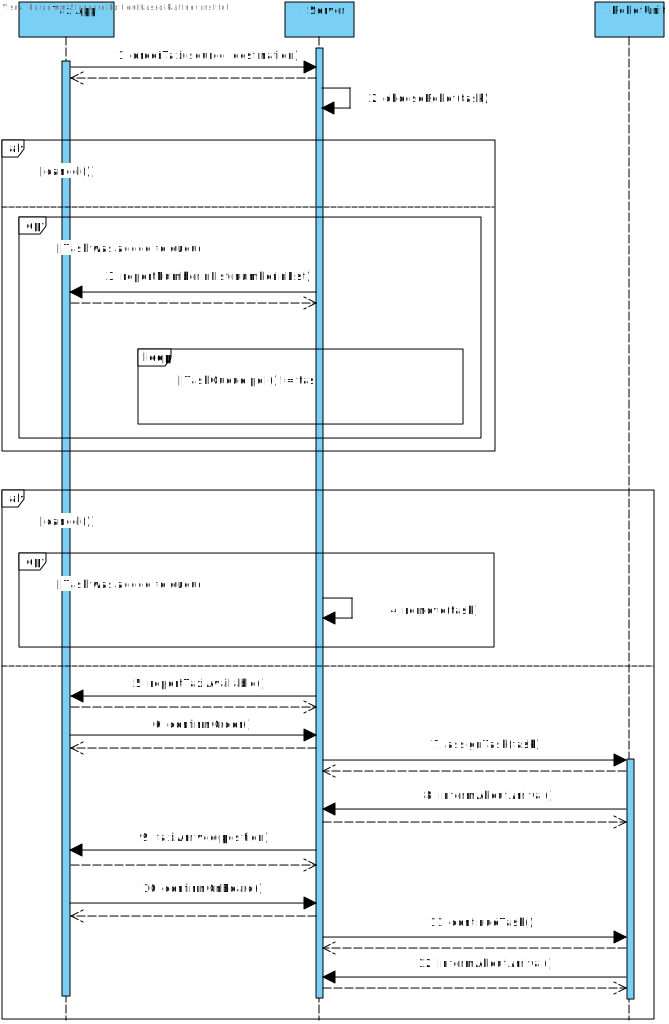
\includegraphics[width=1\textwidth]{img/2-Entwurf-ReceiveOrder-Taxi}
	\caption{\emph{ReceiveOrder}-Sequenzdiagramm, falls ein Kunde ein Taxi anfragt}
	\label{SequenzDiagrammInteraktionTaxi}
\end{figure}

\subsection*{Interaktion zwischen Hospital, Server und RobotUnit}
Der Use Case \texttt{Receive Order} (Use Case 1.1) ermöglicht es nicht nur Taxikunden mit der \emph{TaxiApp} Aufträge an das System zu senden, sondern gibt auch dem \emph{Hospital} die Möglichkeit, Krankentransporte anzufordern. \\
Generell werden Krankenentransporte priorisiert behandelt, sodass, falls keine \emph{RobotUnit} verfügbar ist, eine Taxifahrt unterbrochen wird. Daraus ergibt sich, dass der nachfolgende Prozess ohne eine Warteliste auskommt. \\
Dieser Prozess der Interaktion des \emph{Hospitals}, des \emph{Servers} sowie der \emph{RobotUnits} ist in Abbildung \ref{SequenzDiagrammInteraktionHospital} dargestellt.
Stellt das \emph{Hospital} eine Anfrage, selektiert der \emph{Server} daraufhin eine geeigneten \emph{RobotUnit} und übermittelt ihr den \emph{Task}. \\
Nach der möglichst schnellen Ankunft informiert die \emph{RobotUnit} analog zum Ablauf einer Taxibestellung, den \emph{Server} über seine Ankunft am \emph{Patient}. Diese Information wird an das \emph{Hospital} weitergeleitet, damit dieses das Verladen des \emph{Patients} auf die \emph{RobotUnit} koordinieren kann. \\
Befindet sich der \emph{Patient} an Bord, ruft das \emph{Hospital} im 5. Schritt den Use Case \texttt{Receive Boarding Confirmation} (Use Case 1.3) auf. Der \emph{Server} kann daraufhin der \emph{RobotUnit} den Befehl erteilen, seine Fahrt fortzusetzen. Um das Wohl des \emph{Patients} zu gewährleisten, fährt die \emph{RobotUnit} möglichst vorsichtig zum \emph{Hospital}. \\
Zum Entladen des \emph{Patients} ruft der \emph{Server} auf dem \emph{Hospital} nach Ankunft der \emph{RobotUnit} am \emph{Hospital} die Methode \texttt{informRobotArrivedAtHospital()} auf. Das \emph{Hospital} bestätigt durch Aufrufen des Use Cases \texttt{Receive Unload Confirmation} (Use Case 1.4) im 10. Schritt die Entgegennahme des \emph{Patients}. Die \emph{RobotUnit} steht daraufhin wieder zur Verfügung.
\begin{figure}[H]
	\centering
	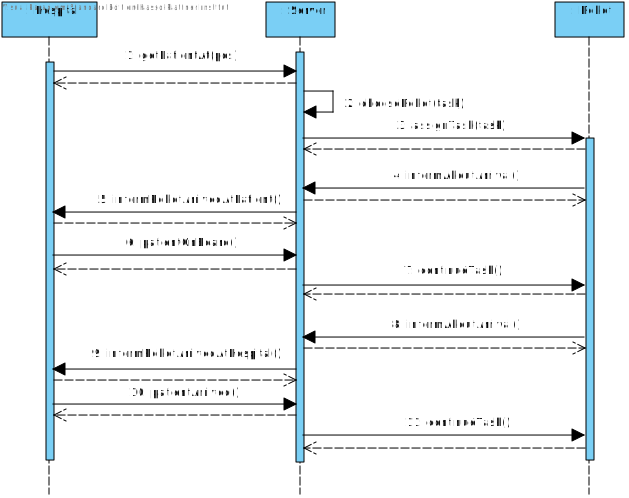
\includegraphics[width=1\textwidth]{img/2-Entwurf-ReceiveOrder-Hosp}
	\caption{\emph{ReceiveOrder}-Sequenzdiagramm, falls das Hospital einen neuen Patienten meldet}
	\label{SequenzDiagrammInteraktionHospital}
\end{figure}


